\chapter{Open Problems: Status and Approaches}
\label{ch:open}

This chapter is the working document of the program. For each open problem it gives the statement, what is known, what we have computed in the course of writing, the approaches that seem promising, and the bearing on the thesis. The problems are numbered for reference. Several have moved since the first draft of this book, and the computations reported here, on near solutions, on connectivity, and on the finite size correction to Simkin\index{Simkin's theorem}, are new.

\section{Problems on the structure of the queens landscape}

\begin{problem}[The low energy ratio]
Compute or prove the existence of $\lim_{N \to \infty} N(0) / N(1)$, the ratio of solutions to placements with exactly one attacking pair.
\end{problem}

Status. We have computed $N(1)$ exactly for $N \le 13$ by backtracking over permutations with at most one conflict. The values and the ratio are in Table~\ref{tab:n1}. The ratio is irregular for small $N$, with $N(1) = 0$ at $N = 5$, and settles from $N = 10$ onwards near $0.04$: $0.050, 0.040, 0.041, 0.039$ for $N = 10$ to $13$. The chain estimates of Chapter~\ref{ch:experiments2} give $N(0)/(N(0) + N(1))$ of about $0.018$ at $N = 32$, which is a ratio $N(0)/N(1)$ near $0.018$, suggesting a slow decrease from $0.04$ at $N = 13$. A heuristic: a solution has $N$ queens and $\binom{N}{2}$ pairs, and a placement with one attack is obtained from a solution by moving one queen so as to create exactly one attack, which can be done in about $cN$ ways for a constant $c$, with the same near solution reachable from about $c'$ solutions; this predicts $N(1) / N(0) \approx (c/c') N$ and a ratio decreasing like $1/N$, which is consistent with $0.04$ at $N = 13$ and $0.018$ at $N = 32$ if $c/c' \approx 2$. Whether the ratio goes to zero like $1/N$ or to a positive constant is the question, and the data to $N = 32$ favour $1/N$.

\begin{table}[t]
\centering
\small
\caption{Exact counts of solutions $N(0)$ and of placements with exactly one attacking pair $N(1)$, the ratio, and the swap connectivity of the level set $\{ S \le 1 \}$: the number of connected components under swaps, the number of components containing a solution, the size of the largest solution containing component, and the number of solutions from which no single swap reaches another solution.}
\label{tab:n1}
\begin{tabular}{rrrrrrrr}
\toprule
$N$ & $N(0)$ & $N(1)$ & ratio & comps & with sol & largest & isolated \\
\midrule
4 & 2 & 8 & 0.250 & 2 & 2 & 1 & 2 \\
5 & 10 & 0 & & 10 & 10 & 1 & 10 \\
6 & 4 & 60 & 0.067 & 10 & 4 & 1 & 4 \\
7 & 40 & 152 & 0.263 & 22 & 6 & 16 & 32 \\
8 & 92 & 888 & 0.104 & 1 & 1 & 92 & 76 \\
9 & 352 & 3376 & 0.104 & 69 & 5 & 348 & 264 \\
10 & 724 & 14404 & 0.050 & 253 & 1 & 724 & 532 \\
11 & 2680 & 67656 & 0.040 & 1121 & 1 & 2680 & 1776 \\
12 & 14200 & 346088 & 0.041 & 4021 & 5 & 14196 & 8668 \\
13 & 73712 & 1910080 & 0.039 & 13257 & 57 & 73656 & 37704 \\
\bottomrule
\end{tabular}
\end{table}

\begin{problem}[Connectivity of solutions under swaps]
Characterise the connected components of $\{ S \le 1 \}$ under swaps of two queens, and in particular whether the solutions lie in one component.
\end{problem}

Status. Resolved for $N \le 13$ by exact computation, with a surprising answer. Table~\ref{tab:n1} shows that although most solutions are isolated under direct swaps, in the sense that no single swap of a solution yields another solution, with $8668$ of $14200$ isolated at $N = 12$ and $37704$ of $73712$ at $N = 13$, almost all solutions lie in a single connected component of $\{ S \le 1 \}$ when swaps are allowed to pass through placements with one attacking pair. At $N = 8$, $10$ and $11$ every solution is in one component. At $N = 12$ all but four of the $14200$ solutions are in one component, and at $N = 13$ all but $56$ of the $73712$. The level set $\{ S \le 1 \}$ has thousands of components, but almost all of them contain no solution; they are small clusters of near solutions that cannot be repaired by a swap. The solutions themselves, bridged by near solutions, form one giant component\index{giant component} with a handful of stragglers.

Conditioned boards. Since the first draft we have also run the connectivity computation on conditioned boards, the case that matters. For $N = 13$ to $17$ we fixed $k = 2$ to $5$ queens of a random solution, enumerated every completion with at most one attacking pair by backtracking, and found the components of this conditioned level set under swaps of the free rows. Table~\ref{tab:conditioned} gives the averages over random instances. The giant component persists: on every instance at every $N$ the largest solution containing component holds at least $96\%$ of the completions, and on most instances all of them. At $N = 13$ with heavier conditioning, $k = 4$ to $8$ fixed queens, the number of completions drops to a handful and the question degenerates, with instances having two completions in separate components; this is the small count regime, not shattering. Random conditioning by queens of a solution does not break the giant component at these sizes, and the ratio $N(0)/N(1)$ on conditioned boards, about $0.03$, matches the unconditioned value. Random conditioning not derived from a solution is another matter, and Section~\ref{sec:depth} shows that such boards have more than one solution component on about half of the boards with two to four fixed queens at $N = 12$, with the giant fraction falling to $11$ to $20$ percent on the worst, against a minimum giant fraction of $0.96$ for solution derived conditioning.

\begin{table}[t]
\centering
\small
\caption{Conditioned boards: $k$ queens of a random solution fixed, the remaining rows free. Averages over random instances of the number of completions $N(0)$, near completions $N(1)$, components containing a completion, and the fraction of completions in the largest such component (mean and minimum over instances).}
\label{tab:conditioned}
\begin{tabular}{rrrrrrrr}
\toprule
$N$ & $k$ & instances & $N(0)$ & $N(1)$ & comps & giant mean & giant min \\
\midrule
13 & 2 & 12 & 510 & & 2.5 & 0.996 & 0.964 \\
14 & 2 & 8 & 2322 & 71574 & 1.25 & 1.000 & 1.000 \\
15 & 3 & 8 & 1163 & 36061 & 2.12 & 0.998 & 0.988 \\
16 & 4 & 6 & 900 & 26658 & 1.17 & 1.000 & 0.999 \\
17 & 5 & 6 & 488 & 14901 & 1.33 & 0.999 & 0.997 \\
\bottomrule
\end{tabular}
\end{table}

The giant component of the unconditioned level set is the structural fact behind the polynomial mixing observed in Chapter~\ref{ch:experiments2}, and it is a strong result for the unconditioned problem: the bottom rung of the ladder is connected, with the exceptions being a vanishing fraction, and the chain can in principle reach every solution from every other. The stragglers, the solutions outside the giant component, cannot be reached by the chain at all, and the sampler is biased by their fraction, which is $4 / 14200$ at $N = 12$ and $56 / 73712$ at $N = 13$; whether this fraction stays negligible is the next question. The conjecture of Chapter~\ref{ch:swendsen} for unconditioned boards is now supported by exact computation to $N = 13$. For conditioned boards the giant component persists under solution derived conditioning to $N = 17$, as described above, while under random conditioning at $N = 12$ about half of the boards with two to four fixed queens have more than one solution component, as described in Section~\ref{sec:depth}.

\begin{problem}[The repair neighbourhood]
Does every solution have $\Omega(N)$ swaps that create at most one attack, and what fraction of all $\binom{N}{2}$ swaps are repairable on average?
\end{problem}

Status. Computed exactly for $N = 6$ to $12$ over every solution. Table~\ref{tab:repair} gives the mean, minimum and maximum number of repairable swaps per solution and the mean as a fraction of all swaps. The fraction is remarkably stable at about $11$ to $12\%$ from $N = 9$ onward, so that the average solution has about $0.115 \binom{N}{2}$ repairable swaps, quadratic in $N$ and far more than the linear count conjectured in Chapter~\ref{ch:mixingproof}. The independence heuristic of that chapter predicted $5/16 = 31\%$; the true fraction is about a third of that, the diagonals through a swap's two new squares being positively dependent. The minimum, however, is small, between $0$ and $2$, and at $N = 12$ there are four solutions with no repairable swap at all. These are exactly the four stragglers outside the giant component in Table~\ref{tab:n1}. So the conjecture is true on average with a quadratic count and false as a statement about every solution: a vanishing fraction of solutions are totally isolated. For the mixing proof this means that lemma one of Chapter~\ref{ch:mixingproof} must be stated for all but an exceptional set, and the exceptional set is the set of stragglers.

\begin{table}[t]
\centering
\small
\caption{Repairable swaps per solution: swaps of two rows that leave at most one attacking pair. Exact over all $Q(N)$ solutions.}
\label{tab:repair}
\begin{tabular}{rrrrrrr}
\toprule
$N$ & $Q(N)$ & mean & min & max & fraction of swaps & solutions with none \\
\midrule
6 & 4 & 0.0 & 0 & 0 & 0.000 & 4 \\
7 & 40 & 2.0 & 1 & 4 & 0.095 & 0 \\
8 & 92 & 3.9 & 2 & 8 & 0.140 & 0 \\
9 & 352 & 4.0 & 2 & 7 & 0.112 & 0 \\
10 & 724 & 5.5 & 2 & 10 & 0.123 & 0 \\
11 & 2680 & 6.5 & 2 & 12 & 0.118 & 0 \\
12 & 14200 & 7.5 & 0 & 16 & 0.114 & 4 \\
\bottomrule
\end{tabular}
\end{table}

\begin{problem}[Finite size correction to Simkin]
Determine the polynomial correction in $Q(N) / N! \sim C N^\beta e^{-(\alpha - 1) N}$.
\end{problem}

Status. We fitted $\log Q(N) - \log N!$ to $c + \beta \log N - a N$ on the exact counts for $N = 12$ to $27$. The free fit gives $a = 0.948$, hence $\alpha = 1.948$, within two of Simkin's error bars of his $1.942 \pm 0.003$, and $\beta = 0.12$. Fixing $a = 0.942$ at Simkin's value gives $\beta = 0.007$ and $c = 0.857$, so $C \approx 2.36$. The near zero value $\beta = 0.007$ is, however, an artifact of pinning $a$ at the central value: fixing $a$ at the ends of Simkin's interval, $0.939$ and $0.945$, gives $\beta = -0.049$ and $0.063$, and the free fit gives $0.12$, so the data bound $|\beta|$ only to about $0.1$. The polynomial correction is therefore not excluded, and $Q(N) \approx 2.4 \, N! \, e^{-0.942 N}$ is a fit, not a finding. The natural conjecture is $\beta = 0$ and $C$ a constant to be identified, which we do not prove; and a second order large deviations analysis around the queenon\index{queenon} would decide it.

\begin{problem}[The queenon and the Lorenz curve]
Determine the limiting normalised staircase $u \mapsto \lim_N \Lambda_N(u)^{1/N}$ and relate it to the queenon.
\end{problem}

Status. Open. The density of states\index{density of states} for $N \le 13$ gives the staircase exactly, and its logarithm divided by $N$ at the energy levels $s/N$ should converge to a rate function $I(e)$ for the energy density $e = s/N$, with $I(0) = \alpha - 1$. A fit of $-\log(N(s)/N!) / N$ against $s/N$ for $N = 10$ to $13$ shows a convex curve with minimum near $e = 2/3$. At $e = 0$ the exact values are $0.852$, $0.874$, $0.869$ and $0.873$ for $N = 10$ to $13$, not yet $0.942$; the gap is the $\log C / N$ term of the finite size problem above, so the endpoint is compatible with Simkin's $\alpha - 1$ but is not shown to reach it. The full rate function is a large deviations problem for the number of attacking pairs in a random permutation, and it should be accessible by the methods of Simkin's upper bound applied at every energy, that is, by a queenon with a prescribed attack density. We have not done this.

\begin{problem}[Mixing on queens level sets]
Determine for which $m = m(N)$ the swap chain on $\{ S \le m \}$ mixes in polynomial time.
\end{problem}

Status. For the unconditioned problem the experiments of Chapter~\ref{ch:experiments2} give autocorrelation time growing like $N^{1.8}$ on $\{ S \le 1 \}$ up to $N = 32$, and the connectivity computation above shows that the solution component is giant up to $N = 13$. A proof of polynomial mixing on $\{ S \le 1 \}$ for the unconditioned problem is plausible and would proceed by canonical path\index{canonical paths}s through the giant component, routing between any two solutions along a path of near solutions; the congestion bound would need a structural understanding of how near solutions are shared, which the $1/N$ heuristic for the ratio suggests. For conditioned boards the question is at least as hard as $\NP = \RP$ and we expect torpid\index{torpid mixing}ity.

\begin{problem}[Mixing of the bottom rung on conditioned boards]
Implement the Gent Jefferson Nightingale reduction and measure the mixing of the swap chain on the resulting boards.
\end{problem}

Status. Not done. This is the single most informative experiment available and we recommend it to anyone taking up the program. The reduction is described in Chapter~\ref{ch:npcomplete} and in the original paper; its implementation requires care with the wall gadgets but no new ideas.

\begin{problem}[The random queens completion model]
Fix $k$ queens uniformly at random subject to pairwise non attack, condition on a completion existing, and determine the satisfiability threshold in $k/N$ and the structure of the completions below it.
\end{problem}

Status. First results at $N = 12$, thirty random instances per $k$, with every completion and near completion enumerated. Table~\ref{tab:randomcompletion} gives the fraction of instances with a completion, the mean number of completions among those, the mean number of swap components containing a completion, the mean and minimum fraction of completions in the largest component, and the number of instances with more than one solution component.

\begin{table}[t]
\centering
\small
\caption{The random queens completion model at $N = 12$: $k$ queens fixed at random, thirty instances per $k$.}
\label{tab:randomcompletion}
\begin{tabular}{rrrrrrr}
\toprule
$k$ & satisfiable & mean $N(0)$ & comps & giant mean & giant min & multi \\
\midrule
1 & 30/30 & 1152 & 3.7 & 0.996 & 0.952 & 22 \\
2 & 30/30 & 110 & 3.0 & 0.960 & 0.795 & 17 \\
3 & 30/30 & 16.5 & 2.7 & 0.818 & 0.222 & 13 \\
4 & 24/30 & 3.7 & 1.9 & 0.755 & 0.250 & 14 \\
5 & 11/30 & 1.4 & 1.1 & 0.955 & 0.500 & 1 \\
6 & 5/30 & 1.2 & 1.0 & 1.000 & 1.000 & 0 \\
7 & 1/30 & 1.0 & 1.0 & 1.000 & 1.000 & 0 \\
\bottomrule
\end{tabular}
\end{table}

Two things appear that the solution derived conditioning of Table~\ref{tab:conditioned} did not show. There is a satisfiability threshold: with $k = 4$ random queens one instance in five has no completion, with $k = 5$ two in three, and with $k = 7$ nearly all, so that at $N = 12$ the threshold is near $k / N \approx 0.35$ to $0.4$. And below the threshold the giant component erodes as $k$ increases: at $k = 1$ it holds $99.6\%$ of completions, at $k = 3$ only $82\%$ on average with instances as low as $22\%$, and at $k = 4$ only $75\%$. Random conditioning that is not derived from a solution does fragment the completions near the threshold, in the manner of the clustering transition of random satisfiability. The counts are small and $N = 12$ is far from asymptotic, so the observation is a pointer rather than a result; the experiment at $N = 16$ to $20$ with chain based estimates where enumeration fails is the obvious continuation, and the quantity to track is the giant fraction at $k / N$ just below threshold as $N$ grows.

\begin{problem}[The physics transition]
Locate the temperature at which the energy fluctuations of the queens Boltzmann model peak.
\end{problem}

Status. Resolved for $N = 8$ to $11$ with a negative answer. From the exact density of states, $\Var_{\pi_\gamma}(S)$ as a function of the inverse temperature $1/\gamma \ge 0$ is maximal at $1/\gamma = 0$ and decreases monotonically as the temperature falls, for every $N$ from $8$ to $11$; Figure~\ref{fig:transition} shows $\Var(S)/N$, which starts near $0.65$ at infinite temperature and falls smoothly to zero. There is no peak at finite positive temperature and so no transition in the thermodynamic sense: the queens Boltzmann model on permutations is, at these sizes, paramagnetic. The difficulty of the counting problem is not a finite temperature phase transition of the kind that stops Swendsen Wang on the Potts model; it is the zero temperature structure of the ground state, its rarity and its connectivity, with no thermodynamic signal on the way down. For the choice of energy domain sampler this means that the multicanonical and $1/k$ ensembles have nothing to fix in the bulk and should be judged entirely by their behaviour at the bottom rung.

\begin{figure}[t]
\centering
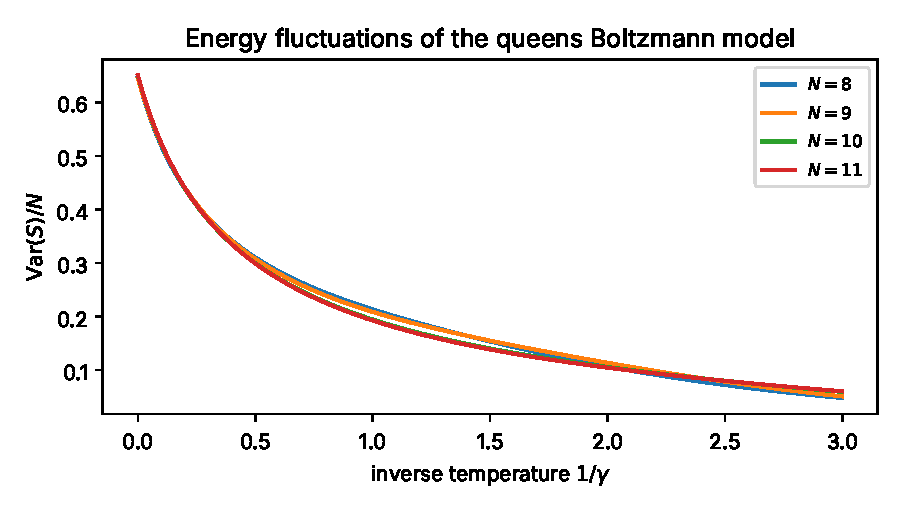
\includegraphics[width=0.85\textwidth]{fig_transition.pdf}
\caption{Energy fluctuations $\Var(S)/N$ of the queens Boltzmann model against inverse temperature, from the exact density of states for $N = 8$ to $11$. The variance is monotone; there is no finite temperature peak.}
\label{fig:transition}
\end{figure}

\section{Problems on the vertical method}

\begin{problem}[The optimal vertical weight]
Characterise the minimax weight $\Omega$ over staircases with $K$ steps and widths in a given range.
\end{problem}

Status. Partially resolved by Chapter~\ref{ch:beyond}: for staircases the stratified\index{stratified sampling} midpoint rule with uniform $\Omega$ is unbiased with mean squared error at most $K \lambda_1^2 / (4n^2)$. We conjecture that no rule can do better than order $K/n^2$ for a staircase with $K$ unknown jump locations, since each jump must be localised to $O(1/n)$ by some node, but we do not prove this lower bound. The constant is open, and the question whether a nonuniform $\Omega$ concentrated near $s = 0$ improves the constant for geometrically decreasing widths, as the queens have, is open.

\begin{problem}[Rates in the quantile coordinate]
Determine the exact dependence of the total error on $K$, $n$ and $\epsilon$ for a staircase whose widths are estimated with relative error $\epsilon$.
\end{problem}

Status. Upper bounds in order of magnitude are given by Chapters~\ref{ch:yakowitz} and~\ref{ch:beyond}, with matching lower bounds not proved: quadrature $O(\sqrt K / n)$, positional $O(\sqrt{\log(1/\rho) / n})$, sampling $O(K \delta)$, the first and third additive and the second relative, in root mean square. The constants are explicit in the stratified case and in the Rao Blackwell\index{Rao Blackwellisation}ised nested case.

\begin{problem}[Two sided promises]
Extend the vertical analysis to $\BPP$.
\end{problem}

Status. Open. The obstacle is that the search to decision reduction of Chapter~\ref{ch:theorems} uses the one sided promise to keep the prefix extension within the promise. For a two sided promise one would need to decide, from a prefix, whether the conditional density is at least $2/3$ or at most $1/3$, and this is a $\BPP$ question again. The known route from $\RP$ to $\BPP$ derandomization is through Andreev, Clementi and Rolim, who show that a hitting set\index{hitting set} generator suffices for $\BPP$ by a nontrivial argument, and the vertical analogue of their argument is not obvious.

\begin{problem}[Hashing versus walking]
Compare the sample complexity of Stockmeyer\index{Stockmeyer's theorem}'s hashing estimator with the vertical walk when both use the same level set sampler\index{level set sampler}.
\end{problem}

Status. Open. With a sampler in place of the $\NP$ oracle, the hashing estimator at hash length $k$ needs to estimate $|S \cap h^{-1}(0)|$, and sampling from $S$ and checking the hash does not do this, since for a pairwise independent $h$ a uniform draw lands in $h^{-1}(0)$ with probability about $2^{-k}$ whatever $|S|$ is, so it estimates the fraction $|S \cap h^{-1}(0)|/|S|$ and carries no information about $|S|$; near the critical length the hit rate is about $1/|S|$ and $O(1/\epsilon^2)$ samples per length do not suffice. We have therefore not completed the comparison, and an earlier estimate of $O(\log|S|/\epsilon^2)$ samples for hashing against $O(K^2/\epsilon^2)$ for the walk should not be relied on. In any case a uniform sampler on $S$ is what hashing needs, and a uniform sampler on $S$ is the bottom rung of the walk, and the walk is the method for producing it. The natural hybrid, which we do not analyse, is to walk to the bottom and hash there, which is what the Jerrum Valiant\index{Valiant, Leslie} Vazirani self reducib\index{self reducibility}ility route does in effect.

\section{Problems on derandomization}

\begin{problem}[Vertical hitting sets]
Find a class of $\RP$ problems beyond $\Pc$ for which the dense level set can be hit by an explicit polynomial size set.
\end{problem}

Status. Open, and by Kabanets and Impagliazzo\index{Kabanets and Impagliazzo} (2004) a deterministic polynomial time algorithm for polynomial identity testing of general arithmetic circuits would imply either that $\mathrm{NEXP} \not\subseteq \Ppoly$ or that the permanent has no polynomial size arithmetic circuits; restricted classes carry no such implication, and explicit hitting sets are known for several (sparse polynomials, by Klivans and Spielman in 2001, and read once oblivious branching programs). One class where this is unconditional is $\mathrm{AC}^0$ by Nisan's generator; the vertical walk for an $\RP$ algorithm whose acceptance predicate is in $\mathrm{AC}^0$ can be derandomized by running it on the $n^{\mathrm{polylog}(n)}$ outputs of Nisan's generator (seed length $\mathrm{polylog}(n)$ for fixed depth), which is quasipolynomial. The polynomial case is open even for $\mathrm{AC}^0$.

\begin{problem}[Deterministic level set hitting for the queens]
Give a deterministic polynomial time procedure that outputs a permutation with at most $m$ attacking pairs for the smallest possible $m$.
\end{problem}

Status. Resolved for the unconditioned problem and open for the conditioned one. Explicit solutions, $m = 0$, are known for all $N \ge 4$: for $N$ coprime to $6$ the permutation $x_i = 2i \bmod N$ is a solution, and Pauls in 1874 and many since have given constructions for all $N$. So the unconditioned level set $\{ S = 0 \}$ is hit deterministically in $O(N)$ time, and the question has content only on conditioned boards, where it is the search version of the $\NP$ complete completion problem.

\section{Problems on the broader program}

\begin{problem}[The Jerrum Valiant Vazirani gap]
Exhibit a non self reducible counting problem for which approximate counting is in $\RP$ but sampling is not known to be.
\end{problem}

Status. Open. Candidates are counting problems defined by non monotone constraints where the self reducibility tree has no uniform structure. The vertical walk counts by sampling level sets, not solutions, and so applies to such problems, but whether it gives an FPRAS\index{FPRAS} without a solution sampler at the bottom is unclear, since the bottom rung is a solution sampler.

\begin{problem}[Lean and the queens]
Formalise the Lorenz\index{Lorenz curve} identity, the product estimator variance bound, and the conditional FPRAS theorem.
\end{problem}

Status. Statements written, proofs open; see Chapter~\ref{ch:lean}, which gives Lean style statements and proof sketches that have not yet been machine checked. The statements are elementary and the main equivalence of Chapter~\ref{ch:theorems} is an assembly of cited theorems; formalising the assembly, with the cited results as axioms, would be a modest project and would produce a machine checked statement of exactly what the program claims.

\section{The shattering depth}
\label{sec:depth}

The third round of computation for this chapter asked a question that the earlier rounds had not: when the bottom level set $\{ S \le 1 \}$ of a board shatters, does the next level set $\{ S \le 2 \}$ shatter too? The answer, on every unconditioned board we have examined, is no, and it changes what the program should ask for.

\begin{problem}[Swap connectivity of the second level set]
Determine the least $m_c(N)$ such that $\{ S \le m_c \}$ is connected under swaps for the unconditioned $N$ queens problem.
\end{problem}

Status. Resolved for $N \le 11$ by exhaustive enumeration of all $N!$ placements with a breadth first search over swaps at every energy threshold. Table~\ref{tab:levelsets} gives the number of swap components of $\{ S \le m \}$ for $m = 0, 1, 2$. The level set $\{ S \le 2 \}$ is connected for every $N$ from $4$ to $11$, so $m_c(N) \le 2$ in this range, and $m_c(N) = 2$ except at $N = 8$, where $\{ S \le 1 \}$ is already connected. At $m = 1$ the level set has many components for $N \ge 9$ ($69$, $253$ and $1121$ for $N = 9$, $10$, $11$), almost all of them small clusters of near solutions containing no solution, as the earlier table showed; at $m = 2$ every one of them is absorbed into a single component. We conjecture that $m_c(N) = 2$ for all $N \ge 9$. The conjecture is needed in the sketch of the conditional FPRAS for $Q(N)$ in Chapter~\ref{ch:program}, where it replaces an argument from monotonicity that the first draft of that proof wrongly relied on: the level sets are nested but the connectivity of a larger one does not follow from the connectivity of a smaller one, and the computation is what supports the claim.

\begin{table}[t]
\centering
\small
\caption{Swap components of the level sets $\{ S \le m \}$ of the unconditioned problem, by exhaustive enumeration. For each $N$: the size of $\{ S \le m \}$ and the number of swap components, for $m = 0$, $1$ and $2$. The level set $\{ S \le 2 \}$ is connected for every $N$ shown.}
\label{tab:levelsets}
\begin{tabular}{rrrrrrr}
\toprule
$N$ & $|\{S \le 0\}|$ & comps & $|\{S \le 1\}|$ & comps & $|\{S \le 2\}|$ & comps \\
\midrule
4 & 2 & 2 & 10 & 2 & 16 & 1 \\
5 & 10 & 10 & 10 & 10 & 66 & 1 \\
6 & 4 & 4 & 64 & 10 & 224 & 1 \\
7 & 40 & 36 & 192 & 22 & 872 & 1 \\
8 & 92 & 84 & 980 & 1 & 3844 & 1 \\
9 & 352 & 304 & 3728 & 69 & 20376 & 1 \\
10 & 724 & 612 & 15128 & 253 & 106056 & 1 \\
11 & 2680 & 2128 & 70336 & 1121 & 584024 & 1 \\
\bottomrule
\end{tabular}
\end{table}

A proof of $m_c(N) \le 2$ would be the natural base of a canonical path\index{canonical paths} argument on $\{ S \le 2 \}$. We do not have one. A proof that $m_c(N) \le c$ for some constant $c$ would already have consequences, since the ratio $N(0) / |\{ S \le c \}|$ should then be at least inverse polynomial, of order $N^{-c}$ by the heuristic that each additional attack can be placed in about $N$ ways; a bound $m_c(N) \le cN$ would not, since by the rate function of Chapter~\ref{ch:entropy} the ratio $N(0) / |\{ S \le cN \}|$ is then exponentially small. The paragraph below explains why the distinction matters.

\begin{problem}[The shattering depth of a board]
For a board $B$ with completions, define the solution depth $m_s(B)$ as the least $m$ such that all completions of $B$ lie in one swap component of the conditioned level set $\{ S \le m \}$, and the shattering depth $m_c(B)$ as the least $m$ such that $\{ S \le m \}$ is itself connected. Determine the distributions of $m_s(B)$ and $m_c(B)$ over random boards and their growth over hard boards.
\end{problem}

Status. The random queens completion model of the previous section showed that random conditioning fragments $\{ S \le 1 \}$. We have now run that model on $300$ instances per $k$ at $N = 12$ and $150$ at $N = 13$, with the fixed queens chosen uniformly subject to pairwise non attack and the instance kept if it has a completion, and the results are in Table~\ref{tab:random2}. About half of the random boards with two to four fixed queens have their completions in more than one component of $\{ S \le 1 \}$: $47\%$ at $N = 12$ with $k = 2$, $62\%$ with $k = 3$, and $54\%$ to $57\%$ at $N = 13$ with $k = 3$ and $4$. The worst boards are severely shattered. A board at $N = 12$ with two fixed queens, at row $0$ column $2$ and row $11$ column $0$, has $42$ completions spread over $30$ components of $\{ S \le 1 \}$, the largest holding $5$ (this board comes from a separate random draw of boards at the same size, not from the $300$ instances of the table, whose most shattered board at $N = 12$ with $k = 2$ has $22$ components); a board at $N = 13$ with three fixed queens has $17$ completions in $15$ components. A greedy adversarial search that moves one fixed queen at a time to increase the number of solution components finds, at $N = 12$ with three fixed queens, a board with $16$ completions in $12$ components and one with $39$ completions in $13$, and with four fixed queens a board whose six completions are all isolated from one another. Shattering of the bottom level set is therefore not rare under random conditioning and can be made severe by a weak adversary, at sizes where the solution derived conditioning of Table~\ref{tab:conditioned} shows nothing of the kind. This is the planted versus random distinction of the satisfiability literature appearing in the queens: a board that was cut out of a solution keeps that solution's component intact, and a board that was not has no such guarantee.

\begin{table}[t]
\centering
\small
\caption{Random boards with $k$ fixed queens and at least one completion, $300$ instances per row at $N = 12$ and $150$ at $N = 13$: mean number of completions, fraction of instances whose completions lie in more than one component of $\{ S \le 1 \}$, mean and maximum number of solution components, and mean and minimum fraction of completions in the largest component.}
\label{tab:random2}
\footnotesize
\begin{tabular}{rrrrrrrr}
\toprule
$N$ & $k$ & mean $N(0)$ & multi & comps & max & giant & min \\
\midrule
12 & 2 & 121.8 & 0.47 & 2.50 & 22 & 0.977 & 0.161 \\
12 & 3 & 15.6 & 0.62 & 2.52 & 11 & 0.826 & 0.111 \\
12 & 4 & 3.2 & 0.46 & 1.63 & 5 & 0.799 & 0.200 \\
12 & 5 & 1.5 & 0.18 & 1.21 & 4 & 0.914 & 0.250 \\
13 & 3 & 59.6 & 0.54 & 2.59 & 15 & 0.944 & 0.118 \\
13 & 4 & 8.7 & 0.57 & 2.22 & 10 & 0.766 & 0.143 \\
13 & 5 & 2.5 & 0.40 & 1.57 & 4 & 0.810 & 0.250 \\
\bottomrule
\end{tabular}
\end{table}

The new fact is what happens one and two levels up. For each of the worst boards we enumerated the conditioned level sets $\{ S \le m \}$ for $m = 2, 3, 4$ and found their swap components. On every one of them all completions lie in a single component of $\{ S \le 2 \}$. The board with $42$ completions in $30$ components of $\{ S \le 1 \}$ has them in one component of $\{ S \le 2 \}$; so does the adversarial board with $39$ completions in $13$ components, and the board with six isolated completions. In every case examined the solution depth is $m_s(B) = 2$: the near solutions with one attack are too sparse to bridge the completions, and the placements with two attacks are dense enough. The level set $\{ S \le 2 \}$ is not itself connected on these boards: it has $94$, $5$ and $13$ components, all but one of them islands of two attack placements that contain no completion. These islands matter, because a chain that samples $\{ S \le 2 \}$ from a completion never reaches them and the fraction of ground states it reports is biased by their mass. One level higher they are absorbed: $\{ S \le 3 \}$ is connected on the first two boards and $\{ S \le 4 \}$ on the third, so the shattering depth is $m_c(B) = 3$ or $4$. On forty random boards with two fixed queens and forty with three, $m_s(B)$ is $1$ on fifteen and $2$ on twenty five of each forty, never more, and $m_c(B)$ is $3$ on seventy five of the eighty, $2$ on three, and $4$ on two. Table~\ref{tab:depth} gives the counts for the three boards, and with them the price of climbing: the ratio $N(0) / |\{ S \le m_c \}|$ is between $0.0005$ and $0.002$ on these boards and about $0.001$ on average over the random ones, against a ratio $N(0) / |\{ S \le 1 \}|$ near $0.04$ on unconditioned boards ($0.039$ at $N = 12$). The price of two levels is a factor of thirty to forty in the bottom ratio, and so of thirty to forty in the number of samples a Bernoulli estimate of that ratio needs.

\begin{table}[t]
\centering
\small
\caption{Depths of three severely shattered boards at $N = 12$. The fixed queens are given as (row, column) pairs; $N(0)$ is the number of completions; for each $m$ the size of the conditioned level set $\{ S \le m \}$, its number of swap components, and the number of those containing a completion. The shattering depth is the first $m$ with one component: $3$, $3$ and $4$. The ratios $N(0) / |\{ S \le m_c \}|$ are $0.0005$, $0.0020$ and $0.0011$.}
\label{tab:depth}
\footnotesize
\begin{tabular}{p{3.2cm}rrrrr}
\toprule
board & $N(0)$ & $m$ & size & comps & with sol \\
\midrule
$(0,2)$, $(11,0)$ & 42 & 1 & 1285 & 447 & 30 \\
 & & 2 & 15549 & 94 & 1 \\
 & & 3 & 87763 & 1 & 1 \\
\midrule
$(7,11)$, $(10,5)$, $(11,10)$ & 39 & 1 & 515 & 98 & 13 \\
 & & 2 & 4335 & 5 & 1 \\
 & & 3 & 19126 & 1 & 1 \\
\midrule
$(0,7)$, $(1,11)$, $(8,10)$, $(11,8)$ & 6 & 1 & 49 & 23 & 6 \\
 & & 2 & 448 & 13 & 1 \\
 & & 3 & 1928 & 2 & 1 \\
 & & 4 & 5265 & 1 & 1 \\
\bottomrule
\end{tabular}
\end{table}

This changes the shape of the mixing conjecture. The vertical walk does not need the bottom rung; it needs some rung whose level set is connected and well mixed and whose ratio to the ground state is not too small. The following statement makes that precise.

\begin{theorem}[Rung skipping]
\label{thm:rungskip}
Let $B$ be a board with completions and let $m \ge m_c(B)$. Suppose the swap chain on the conditioned level set $\{ S \le j \}$ is irreducible and mixes in time $T$, polynomial in $N$, for every $j \ge m$, that $|\{ S \le j \}| / |\{ S \le j + 1 \}| \ge 1 / q(N)$ for every $j \ge m$ and a polynomial $q$, and that $N(0) / |\{ S \le m \}| \ge 1 / p(N)$ for a polynomial $p$. Let $K$ be the number of rungs above $m$, that is, the number of $j \ge m$ with $\{ S \le j \}$ not the whole board. Then the vertical walk that estimates $N(0) / |\{ S \le m \}|$ directly, as the fraction of ground states among samples from $\{ S \le m \}$, and the ratios $|\{ S \le j \}| / |\{ S \le j + 1 \}|$ for $j \ge m$ by the product estimator, is an FPRAS for the completion count with cost $O((K^3 q(N) + p(N)) \epsilon^{-2} T \log (K/\delta))$ for confidence $1 - \delta$.
\end{theorem}

\begin{proof}
The bottom ratio is a Bernoulli mean with success probability at least $1/p(N)$, so $O(p(N) \epsilon^{-2} \log (1/\delta))$ samples give relative error $\epsilon / 2$ with the stated confidence. Each rung ratio $|\{ S \le j \}| / |\{ S \le j + 1 \}|$ above $m$ is a Bernoulli mean, under the uniform law on $\{ S \le j + 1 \}$, of at least $1/q(N)$, by the rung ratio hypothesis, so $O(q(N) K^2 \epsilon^{-2} \log (K/\delta))$ samples from a chain with mixing time $T$ estimate it to relative error $\epsilon / (2K)$, and the product of the $K$ estimates has relative error about $\epsilon / 2$, so that with the bottom ratio the total is within a constant multiple of $\epsilon$, which rescaling $\epsilon$ removes; this is the argument of the conditional FPRAS theorem of Chapter~\ref{ch:program}, run on the conditioned level sets instead of the unconditioned ones. The condition $m \ge m_c(B)$ is necessary rather than sufficient for the mixing hypothesis: below the shattering depth the level set is disconnected and no chain on it is irreducible, and above it irreducibility at every level $j \ge m$ is part of what is assumed, since the connectivity of $\{ S \le m \}$ does not by itself imply that of $\{ S \le m + 1 \}$. Solution depth is not enough: a chain on $\{ S \le m_s \}$ started from a completion samples the completion component uniformly but never the islands, and the ground state fraction it reports is too large by the factor of the island mass.
\end{proof}

The theorem relocates the question. On the boards examined at $N = 12$, $m = 3$ suffices on all but two of eighty, $m = 4$ on those two, and larger $N$ need $m = 4$ more often (Table~\ref{tab:depthgrowth}), and the price is a factor of thirty to forty in the bottom ratio, which is nothing. The mixing conjecture for hard boards is then not that $\{ S \le 1 \}$ shatters, which it demonstrably does on easy random boards as well, but that the shattering depth grows: that on reduction boards from hard formulas $m_c(B)$ is of order $N$ or larger, so that the first connected level set has exponentially more placements than completions and the Bernoulli estimate of the bottom ratio takes exponential time. Equivalently, the hardness lives not in the disconnection of one level set but in the depth to which the disconnection persists. We state this as the revised conjecture.

\begin{conjecture}[Shattering depth on hard boards]
\label{conj:shatterdepth}
There is a family of boards $B_N$ from the Gent Jefferson Nightingale reduction applied to hard formulas with $m_c(B_N) \ge c N$ for a constant $c > 0$, and for such boards the ratio $N(0) / |\{ S \le m_c(B_N) \}|$ is exponentially small in $N$.
\end{conjecture}

The conjecture is testable: the enumeration that found $m_c = 3$ on the random boards runs in seconds at $N = 12$, and on a reduction board of moderate size it would find the depth directly. Its negation at every size, $m_c(B) \le c$ for a constant $c$ on all boards, together with polynomial mixing above the depth, an inverse polynomial bound on $N(0) / |\{ S \le c \}|$ and on the rung ratios, would give $\NP = \RP$ by the rung skipping theorem and the main equivalence, and this is now the sharpest form of the program's Monte Carlo half that we can state: find the shattering depth of hard boards.

\begin{problem}[Queenon tilted proposals]
Does a swap proposal tilted towards the queenon density mix faster than the uniform swap on the bottom level set?
\end{problem}

Status. Resolved negatively at the sizes tested. Simkin\index{Simkin's theorem}'s queenon\index{queenon} is the limiting density of queen positions in a uniform solution, and one might hope that proposing swaps that move queens towards the dense parts of the board would raise the acceptance rate of the bottom rung chain. We estimated the density from the $73712$ solutions at $N = 13$, interpolated it to an $N \times N$ board, and ran the swap chain on $\{ S \le 1 \}$ with the pair $(i, j)$ proposed with probability proportional to $q(i, x_j) \, q(j, x_i)$, the product of the densities at the two squares the swap would occupy, with the Metropolis Hastings correction that keeps the uniform target. Figure~\ref{fig:queenon} shows the density and the comparison. The density is far from flat: along the middle row it is $1.42$ times uniform at the edges and $0.79$ at the centre, and along the top row $0.49$ at the corners and $1.42$ at the centre, the pattern that Simkin's queenon predicts. The tilt does not help. At $N = 12, 16, 20, 24$ the integrated autocorrelation times of the first row column are $246, 402, 775, 716$ proposals for the uniform swap and $312, 489, 956, 761$ for the tilted swap, with standard deviations over five runs of sixteen to forty eight percent, and the acceptance rates fall from $0.061, 0.046, 0.036, 0.032$ to $0.052, 0.040, 0.033, 0.029$. The tilted chain is slightly slower at every size. The reason is that the queenon is a one point marginal and the constraints are pairwise: the squares that are dense are dense because many solutions use them, not because a given near solution can be repaired by moving a queen there, and proposing moves towards them lowers the acceptance rate without shortening the repair paths. A proposal that could help would have to use the conditional density of a square given the other queens, which is the thing the chain is trying to sample. The problem that remains open is whether a two point tilt, using Simkin's bound on the density of attacking pairs, does any better; we expect not.

\begin{figure}[t]
\centering
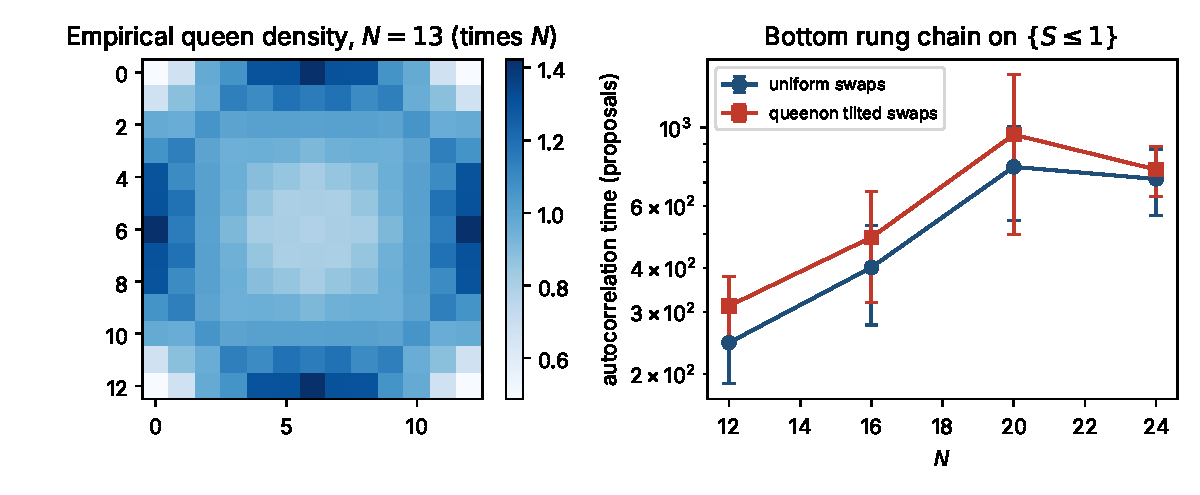
\includegraphics[width=\textwidth]{fig_queenon.pdf}
\caption{Left: the empirical queen density at $N = 13$, from all $73712$ solutions, scaled so that uniform is one. Right: autocorrelation time of the bottom rung chain with uniform and queenon tilted swap proposals, mean and standard deviation over five runs.}
\label{fig:queenon}
\end{figure}


\section{The fourth round: gaps, depths and windows}
\label{sec:round4}

This round carries out three computations that the earlier rounds left open: the spectral gap of the bottom rung chain, the growth of the shattering depth with $N$, and the divergence of the solution law from Markov window families. One of them moved the program's conjecture; one of them showed that a depth of three does not suffice on all boards; and one closed a door that Chapter~\ref{ch:ce} had left ajar.

\begin{problem}[The spectral gap of the bottom rung chain]
Compute the spectral gap of the swap chain on the giant component $G_N$ of $\{ S \le 1 \}$ and its growth with $N$.
\end{problem}

Status. Computed exactly for $N = 8$ to $12$ by a sparse eigensolver on the transition matrix of the chain, which has $980$, $3636$, $14824$, $69096$ and $355860$ states; the last took over an hour, the top of the spectrum being nearly degenerate. Table~\ref{tab:gap} gives the relaxation time $1 / \gamma$ of the chain in proposed swaps, the relaxation time restricted to the subspace of functions invariant under the eight symmetries of the board, which is the one that governs every symmetric observable and in particular the ground state indicator that the walk averages, the conductance of the cut defined by the sign of the second eigenvector, and the symmetry under which the second eigenvector is antisymmetric.

\begin{table}[t]
\centering
\small
\caption{The swap chain on the giant component $G_N$ of $\{ S \le 1 \}$: number of states, relaxation time $1/\gamma$ in proposed swaps, relaxation time on the symmetric subspace, the conductance of the sign cut of the second eigenvector, and the symmetry under which that eigenvector is antisymmetric. The three smallest nonzero eigenvalues of $I - P$ for the lazy chain are $0.00166, 0.00182, 0.00261$ at $N = 8$; $0.001127, 0.001127, 0.001138$ at $N = 9$; $0.000910, 0.000914, 0.000914$ at $N = 10$; $0.000571, 0.000571, 0.000572$ at $N = 11$; and $0.000484, 0.000484$ for the first two at $N = 12$, where the symmetry analysis was not run.}
\label{tab:gap}
\begin{tabular}{rrrrrl}
\toprule
$N$ & states & $1/\gamma$ & symmetric & $\Phi$(cut) & antisymmetric under \\
\midrule
8 & 980 & 301 & 275 & 0.0070 & both reflections \\
9 & 3636 & 444 & 433 & 0.0077 & transpose \\
10 & 14824 & 549 & 547 & 0.0072 & transpose \\
11 & 69096 & 875 & 874 & 0.0073 & half turn \\
12 & 355860 & 1033 & & 0.0060 & \\
\bottomrule
\end{tabular}
\end{table}

Three things are in the table. First, the relaxation time grows faster than the autocorrelation time of Chapter~\ref{ch:experiments2}: the pairwise exponents are $3.3$, $2.0$, $4.9$ and $1.9$ and the least squares exponent over $N = 8$ to $12$ is $3.1$, against the $1.76$ of the first row column to $N = 32$. The two are not in conflict, since the autocorrelation time of one observable is a lower bound for the relaxation time up to a factor of about two and the first row column is far from the slowest function, but the exponent that the expansion conjecture of Chapter~\ref{ch:mixingproof} has to deliver is the larger one. Second, the top of the spectrum is nearly degenerate: at $N = 10$ and $11$ the three smallest nonzero eigenvalues agree to two or three figures, and the second eigenvector is antisymmetric under a board symmetry, the transpose at $N = 9$ and $10$ and the half turn at $N = 11$, while the symmetric subspace relaxes at almost the same rate. The symmetry explains the particular eigenvector and not the slowness. A band of near degenerate slow modes is the spectral signature of many bottlenecks of comparable strength, and the landscape of Chapter~\ref{ch:mixingproof} says what they are: clusters of near solutions attached to the giant component by few swaps. Third, the sign cut of the second eigenvector has conductance between $0.006$ and $0.008$ at every $N$, so it is not the bottleneck; by Cheeger's inequality the true conductance satisfies $\gamma / 2 \le \Phi \le \sqrt{2 \gamma}$, that is, $0.0005 \le \Phi_{12} \le 0.044$, and the bottleneck sets are not symmetry halves but something smaller that the eigenvector does not reveal directly. Finding them is the next step on this problem: the second eigenvector restricted to the symmetric subspace, thresholded at levels other than zero, and the clusters it isolates.

The practical reading is that the expansion conjecture should be stated with $c'$ near $3$ rather than near $2$, that the bottom rung needs of order $N^3$ swaps per effective sample for the worst observable and of order $N^{1.8}$ for the first row column over the range measured, and that the computation at $N = 13$ with a symmetry reduced matrix, which has eight times fewer states, is within reach and would tell whether the pairwise exponents, which swing between $1.9$ and $4.9$, are settling.

\begin{problem}[Growth of the shattering depth]
Determine how $m_c(B)$ grows with $N$ on random boards.
\end{problem}

Status. Measured at $N = 14$ and partly at $N = 16$, with a C implementation of the enumeration that handles level sets of twenty million placements. Table~\ref{tab:depthgrowth} gives the distribution of the solution depth $m_s$ and the shattering depth $m_c$ over the random boards at each $(N, k)$, and the mean ratio $N(0) / |\{ S \le m_c \}|$ at the depth. The fraction of boards that need $m_c = 4$ grows. At $N = 12$ the level set was connected at $m = 3$ on $75$ of $80$ boards (already at $m = 2$ on three more); at $N = 14$ it is connected at $m = 3$ on $22$ of $40$ and needs $m = 4$ on the other $18$, and at $N = 16$ with four fixed queens it is connected at $m = 3$ on one board of eight and needs $m = 4$ on the other seven, while with five fixed queens it is connected at $m = 3$ on three of eight and needs $m = 4$ on the other five. The solution depth does not grow: completions reconnect at $m = 1$ or $2$ at every size. The price grows with the depth, from $1 \times 10^{-3}$ at $N = 12$ to $3 \times 10^{-4}$ at $N = 14$ and $1 \times 10^{-4}$ to $2 \times 10^{-4}$ at $N = 16$, a factor of about three for every two rows. Since $k$ changes with $N$ in the table ($2$ and $3$ at $N = 12$ and $14$, $4$ and $5$ at $N = 16$), the effects of $N$ and of $k$ are confounded.

\begin{table}[t]
\centering
\small
\caption{Growth of the depths with $N$ on random boards with $k$ fixed queens, forty boards per row at $N = 12$, twenty at $N = 14$ and eight at $N = 16$: the number of boards with solution depth $m_s = 1$ and $2$, with shattering depth $m_c = 2$, $3$ and $4$, and the mean of $N(0) / |\{ S \le m_c \}|$ over the boards.}
\label{tab:depthgrowth}
\begin{tabular}{rrrrrrrr}
\toprule
$N$ & $k$ & $m_s{=}1$ & $m_s{=}2$ & $m_c{=}2$ & $m_c{=}3$ & $m_c{=}4$ & mean ratio \\
\midrule
12 & 2 & 15 & 25 & 0 & 39 & 1 & $7.9 \times 10^{-4}$ \\
12 & 3 & 15 & 25 & 3 & 36 & 1 & $1.3 \times 10^{-3}$ \\
14 & 2 & 15 & 5 & 0 & 12 & 8 & $3.0 \times 10^{-4}$ \\
14 & 3 & 13 & 7 & 0 & 10 & 10 & $2.8 \times 10^{-4}$ \\
16 & 4 & 5 & 3 & 0 & 1 & 7 & $1.0 \times 10^{-4}$ \\
16 & 5 & 4 & 4 & 0 & 3 & 5 & $1.7 \times 10^{-4}$ \\
\bottomrule
\end{tabular}
\end{table}

This shows that a depth of three does not suffice on every board measured, and it changes the conjecture. The hypothesis that the depth is bounded on random boards and grows only on reduction boards is no longer clearly the best reading of the data; the typical depth on random boards moves by about one between $N = 12$ and $16$, and the question is whether it keeps moving and at what rate. If $m_c$ grows like $\log N$ the price $N(0) / |\{ S \le m_c \}|$ is only quasi-polynomial, of order $N^{c \log N}$, by the heuristic that each extra attack costs a factor of order $N$, and the rung skipping theorem gives a quasi-polynomial and not a polynomial walk on random boards; only a bounded $m_c$ gives an inverse polynomial price. If $m_c$ grows like $cN$ the price is exponential and the walk fails on random boards, which would place the random queens completion problem with the problems on which Monte Carlo fails on average, and would make the reduction board question moot for this chain. The data to $N = 16$ cannot tell $\log_2 N$ from $N / 4$: rounded down, both give $3$ at $N = 12$ and $4$ at $N = 16$. The measurement that decides is the depth at $N = 20$ and $24$, which the C enumeration can reach for level sets up to about $10^8$ placements, and at those sizes $\log_2 N$ rounded down predicts $4$ and $N / 4$ predicts $5$ to $6$. We state the revised conjecture with the alternative it must beat.

\begin{conjecture}[Depth growth]
\label{conj:depthgrowth}
On random boards with a fixed number of fixed queens, $m_c(B) = O(1)$ with high probability, so that the price of rung skipping is inverse polynomial. The data to $N = 16$ do not exclude slow growth: $m_c(B) = O(\log N)$ would make the price quasi-polynomial, and the alternative, $m_c(B) \ge cN$, would make the vertical walk exponential on random boards.
\end{conjecture}

The unconditioned problem is unaffected: $\{ S \le 2 \}$ is connected for $N \le 11$ with no fixed queens, and the realistic prize of Chapter~\ref{ch:program} rests on the connectivity of $\{ S \le 2 \}$ or on the giant component of $\{ S \le 1 \}$, together with the rung ratio hypothesis of its theorem, and not on the depth of a conditioned board.

\begin{problem}[Markov window families]
Compute the divergence from the uniform law on solutions to its projection on the order $k$ Markov sequential family, as a function of $k$ and $N$.
\end{problem}

Status. Computed exactly for $N = 8$ to $13$ from all solutions. For the family $g(x) = \prod_i g_i(x_i \mid x_{i-k}, \dots, x_{i-1})$ with unrestricted window conditionals, the minimum divergence is
\[
D_k(N) = \sum_{i=1}^N H(X_i \mid X_{i-k}, \dots, X_{i-1}) - \log Q(N) ,
\]
with the window truncated at row $1$ for $i \le k$, by the same entropy decomposition as Theorem~\ref{thm:product} of Chapter~\ref{ch:ce}, the conditional entropies being those of a uniform random solution, and Table~\ref{tab:window} gives it. Two facts are in the table. For fixed window $k$ the divergence grows linearly in $N$: $D_2$ increases by about $2.4$ nats per row and $D_3$ by about $2.9$ from $N = 10$ on, so the information that the diagonal constraints carry beyond any fixed window is more than two nats per queen, and, if the linear growth seen for $N = 8$ to $13$ continues, the relative variance of importance sampling from any such family, at least $e^{D_k} - 1$, is exponential in $N$. And the window needed to bring the divergence below one nat is about half the board: $k = 3, 4, 5, 5, 6, 7$ for $N = 8$ to $13$. This is the cross entropy form of the shattering depth that Chapter~\ref{ch:ce} asked for, and it is linear in $N$. A sequential family whose conditionals see only a window of fixed width, which is what the cross entropy method uses for permutation problems, cannot give a polynomial time counter for the queens; a family whose conditionals see the whole history can, in principle, since $D_{N-1} = 0$, but the representation question of Chapter~\ref{ch:gbc} is then whether a conditional of the full history can be computed by a polynomial size circuit to within $O(\log N)$ nats, and the window computation says the circuit cannot be local.

\begin{table}[t]
\centering
\small
\caption{Divergence $D_k(N)$ in nats from the uniform law on solutions to the best order $k$ Markov sequential family, exact from all solutions, and the least $k$ with $D_k < 1$.}
\label{tab:window}
\begin{tabular}{rrrrrrrrr}
\toprule
$N$ & $Q(N)$ & $D_0$ & $D_1$ & $D_2$ & $D_3$ & $D_4$ & $D_5$ & $k(D_k < 1)$ \\
\midrule
8 & 92 & 11.4 & 7.3 & 3.0 & 0.82 & 0.21 & 0 & 3 \\
9 & 352 & 13.7 & 10.2 & 5.9 & 2.1 & 0.67 & 0.26 & 4 \\
10 & 724 & 16.2 & 12.6 & 8.1 & 3.6 & 1.15 & 0.37 & 5 \\
11 & 2680 & 18.2 & 14.9 & 11.0 & 6.3 & 2.45 & 0.81 & 5 \\
12 & 14200 & 20.0 & 16.8 & 13.3 & 9.7 & 5.13 & 2.03 & 6 \\
13 & 73712 & 21.9 & 18.7 & 15.4 & 12.3 & 8.28 & 4.31 & 7 \\
\bottomrule
\end{tabular}
\end{table}

The three computations point the same way. The chain's relaxation time grows like $N^3$, the fraction of conditioned boards that need the deeper level set grows with $N$, and the window a sequential family needs grows like $N / 2$: on every axis the queens get harder with $N$ faster than the first measurements suggested. Nothing in this round is a proof.

\section{What has moved}

Since the first draft, ten problems have changed status. The repair neighbourhood is quadratic on average and empty for a vanishing set of stragglers. The random completion model shows a satisfiability threshold near $k/N = 0.35$ to $0.4$ at $N = 12$ and, on three hundred instances, a bottom level set that has more than one solution component on about half of the random boards with two to four fixed queens and fragments severely on the worst of them. The physics transition is absent for $N \le 11$. The connectivity problem is resolved for $N \le 13$ with the giant component result on unconditioned boards, which persists under solution derived conditioning to $N = 17$ and does not persist on about half of the boards under random conditioning at $N = 12$. The second level set $\{ S \le 2 \}$ is connected for $N \le 11$ on unconditioned boards; on shattered boards the completions reconnect in $\{ S \le 2 \}$ and the level set itself reconnects at a depth that is two to four at $N = 12$, three or four at $N = 14$, and three or four at $N = 16$ on the boards examined; the data do not yet show that the shattering depth grows with $N$, and if it does the question is whether like $\log N$ or like $N$. The spectral gap of the bottom rung chain is known exactly to $N = 12$: its relaxation time grows like $N^3$, with a nearly degenerate band of slow modes that the board symmetries do not explain. The Markov window a sequential family needs to come within a nat of the solution law is half the board. The queenon tilted proposal does not accelerate the bottom rung. The finite size correction problem has a numerical conjecture, $\beta = 0$ and $C \approx 2.4$, which the fit supports only to $|\beta| \lesssim 0.1$ given Simkin's error bar. The deterministic hitting problem is resolved trivially for unconditioned boards by the explicit constructions. The problems that remain, and that matter most, are two: the rate of growth of the shattering depth on random boards, which decides whether the walk is polynomial on average, and the depth on reduction boards, which decides whether it is polynomial in the worst case. The enumeration that measures both runs in minutes at $N = 16$, and the next sizes are $20$ and $24$.
